\documentclass[]{standalone}

\usepackage
{
	tikz,
	pgfplots,
	verbatim,
	amssymb,
}


\usetikzlibrary
{
	arrows,
	patterns,
	angles,
	quotes,
	calc, 
	3d,
	backgrounds, 
	positioning
}

\begin{document}
	
	\pgfplotsset{
		width=10cm,
		compat=newest,
		every axis/.append style={
			axis x line=middle,
			axis y line=middle,
			enlargelimits=true,
			x=1cm, y=1cm,
			xlabel={$x$},
			xlabel style={below left, scale=1.5},
			ylabel={$y$},
			ylabel style={below right, scale=1.5},
			ymajorgrids=true,
			xmajorgrids=true,
			xticklabels={},
			yticklabels={},
			samples=5000,
			grid=both,
			grid style={thick},
			axis line style={very thick},
			ticks=both,
			xtick={-100,-99,...,100},
			ytick={-100,-99,...,100},
			restrict y to domain=-500:500,
			 % enable layer, needed to draw middle grid below axis
			set layers=standard,
			% disable ticks
			every major tick/.style={draw=none},
			every minor tick/.style={draw=none},
	}}
	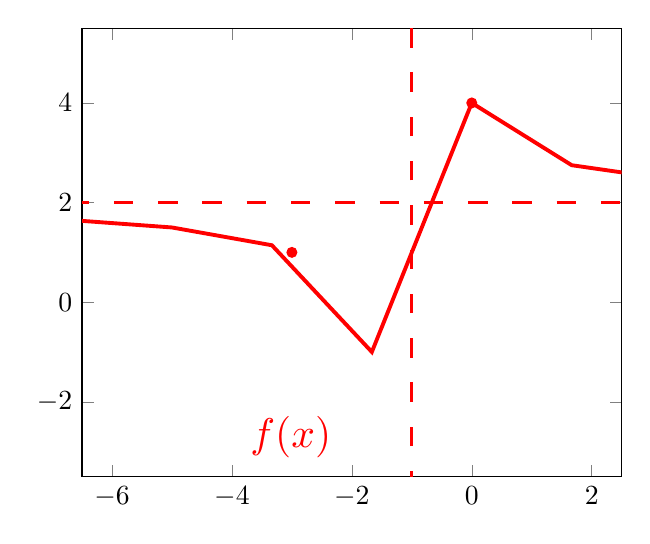
\begin{tikzpicture}[>=stealth, baseline={([yshift={-\ht\strutbox}]current bounding box.north)}]
		\begin{axis}[
			xmin=-6.5,xmax=2.5,
			ymin=-3.5,ymax=5.5,
			ylabel style={below right},]
			\addplot [red,line width=1.4pt,domain=-20:20] {2/(x+1)+2};
			\addplot[red,line width=1.2pt,dash pattern=on 7pt off 9pt,domain=-20:20] {2};
			\draw[red,line width=1.2pt,dash pattern=on 7pt off 9pt,domain=-10:10] (-1,-10)--(-1,10);
			\fill[fill=red] (0,4) circle (2pt);
			\fill[fill=red] (-3,1) circle (2pt);
			\draw (-2.1,-2) node[anchor=north east, red, scale=1.5, fill=white] {$f(x)$};
		\end{axis}
	\end{tikzpicture}
	
\end{document}